

\section{Intermittent Computing} \label{sec:ips}

Energy harvesting provides an autonomous power supply for wireless sensor nodes as an alternative of battery power. However, with small storage, energy harvesting systems inevitably suffer from frequent power outages, which affect forward execution of programs. Intermittent computing (IC, also known as transient computing) aims to maintain forward execution and computation correctness through power failures~\cite{ransford2012mementos}. Intermittent execution spans its execution and intermittently computes over power outages, while conventional execution restarts after power interruptions. A typical characteristic of an IC system is that it starts executing whenever there is power available and suspends during power outages; after power recovery, it can continue its prior task correctly instead of restarting from the beginning of a program. 

Due to different design considerations, the methodologies in IC varies in a wide spectrum~\cite{sliper2018enabling}. 
These methodologies include saving snapshots of system volatile state into NVM, breaking down execution into small tasks, hardware circuits for suspend and restore operations. 
The existing IC approaches can be classified into four types: checkpointing, reactive IC, task-based IC, and non-volatile processors (NVP). 
The following part of this section explains \correct{each of the above methodologies with the associated research progress}.

\subsection{Checkpointing IC}

Checkpointing IC inserts checkpoints into code at compile time. When a checkpoint is called, the system checks the current available energy amount. If this amount is less than a predefined threshold, which indicates the available energy may not be enough to sustain execution, a snapshot saving function is called at this checkpoint. To save a snapshot of the system computing state, the system \correct{copies the } current stacks and heaps, local and global variables, general registers, the stack pointer, and the program counter, into the NVM. A checkpointing system continuously operates until it encounters power outages, where the supply voltage is less than the minimum operating voltage of the systems. After the supply voltage recovers, \correct{the system restores its state from the last checkpoint, and hence, continues its execution from that checkpoint}. 
% a figure here explaining the control flowing of checkpointing?

Mementos~\cite{ransford2012mementos} first presents a checkpointing solution in which checkpoints are placed at design time. 
Mementos includes three strategies \correct{for placing checkpoints}, which are placing at every loop, placing at every function call, and an auxiliary timer delay to determine the minimum cycle between two adjacent checkpoints. 
Additionally, programmers can also insert or delete checkpoints manually as a custom option. 
Two NVM blocks are used and snapshots are saved to the two blocks alternately, so there is always at least one available and complete snapshot even if the energy is depleted during saving a new snapshot. 
One significant shortcoming of Mementos is the instrumenting strategy: with the different sizes of loops and functions, the granularity of checkpoints can be either too small, which introduces high run-time overheads, or too large, which leads to non-termination where the execution can never get to the next checkpoint. 
\correct{Another concern in Mementos is how to set the voltage threshold so that snapshots can be saved successfully while avoiding too many redundant snapshots.}

HarvOS~\cite{bhatti2017harvos} is proposed to improve the strategies of inserting checkpoints in Mementos. HarvOS analyses the control-flow graph of a program and splits it into sub-graphs with a checkpoint inserted for each sub-graph. To reduce the number of checkpoints compared to Mementos, the size of sub-graphs is set close to the worst-case number of useful cycles the MCU can execute until the next checkpoint. To reduce the size of snapshots, the RAM usage in each sub-graph is analysed and the checkpoint is placed at the point with the least RAM usage. HarvOS claims to reduce 68\% checkpoints on average compared to Mementos.

Chinchilla~\cite{maeng2018adaptive} proposes a checkpointing tool which automatically overprovisions checkpoints at compile time and adaptively eliminates unnecessary checkpoints at run time. Compared to Mementos and HarvOS, Chinchilla relieves the programming efforts on manually inserting checkpoints while still achieves an efficient number of checkpoints at run time.

An advantage of the checkpointing method is the size of a specific snapshot can be estimated from the program execution flow to find a smaller snapshot~\cite{bhatti2017harvos}. However, there are still two significant challenges remaining unsolved in checkpointing methods: idempotency violation and non-termination. 

An execution is idempotent if it can be repeated while maintaining the same result~\cite{lucia2015simpler}. Non-idempotent actions include I/O operations and NVM writes, which are fairly common in IC applications. Repeating non-idempotent actions can leads to undesired results, so these non-idempotent actions should be executed only once. Checkpointing systems repeat executing the code between two adjacent checkpoints, and hence, cause non-idempotency. Current compile-time checkpointing methods as listed above are not able to ensure idempotency. 

Non-termination in checkpointing systems exhibits when the energy consumption between two checkpoints is more than the buffered and harvested energy. Non-termination typically happens when the instrumentation strategy of checkpoints ignores the size of the energy buffer, as in Mementos. HarvOS and Chinchilla manage to mitigate non-termination, but they cannot eliminate this problem as they cannot dynamically insert checkpoints at run time according to varying environmental sources. 
% Main drawbacks: idempotency, non-termination/deadlock.

\subsection{Reactive IC} \label{Section:reactiveic}

Instead of instrumenting checkpoints at compile time, reactive IC does not set predefined checkpoints but save snapshots at run time when the supply voltage is detected to be lower than a threshold that indicates an imminent power failure. Therefore, the snapshot saving operations is only invoked when there is an indication of an imminent power outage, i.e. a low supply voltage. Also, after saving a snapshot, a reactive IC system suspends its execution and enter a low-power mode, rather than continues execution until a power outage as checkpointing systems do. When the voltage supply recovers above a restore threshold, the system either restores the last snapshot if the system reboots, or just continues execution if the system comes back from the low-power mode.

Hibernus~\cite{balsamo2015hibernus} saves only one snapshot before a power interruption and then enter the sleep mode. Two fixed voltage thresholds, $V_H$ and $V_R$, are predefined for hibernation (save a snapshot and sleep) and restoring a snapshot. An on-chip voltage comparator and an on-chip voltage reference generator are used for monitoring the supply voltage and triggering hibernation when the supply voltage drops to $V_H$ or restoration when the supply voltage recovers to $V_R$. A voltage trace is shown in~\fref{Figure:hibernus} to explain Hibernus behaviours, and this trace is representative for a reactive IC system behaviours. To adapt thresholds to variable energy sources, Hibernus++~\cite{balsamo2016hibernus++} implements dynamic self-calibration for suspend and restore thresholds by executing a hibernation test. By using adaptive thresholds instead of fixed thresholds as in Hibernus, Hibernus++ makes itself compatible with a variety of energy sources. Compared to Hibernus, Hibernus++ improves application execution time by reducing the overheads of suspend and restore operations.

\begin{figure}
    \centering
    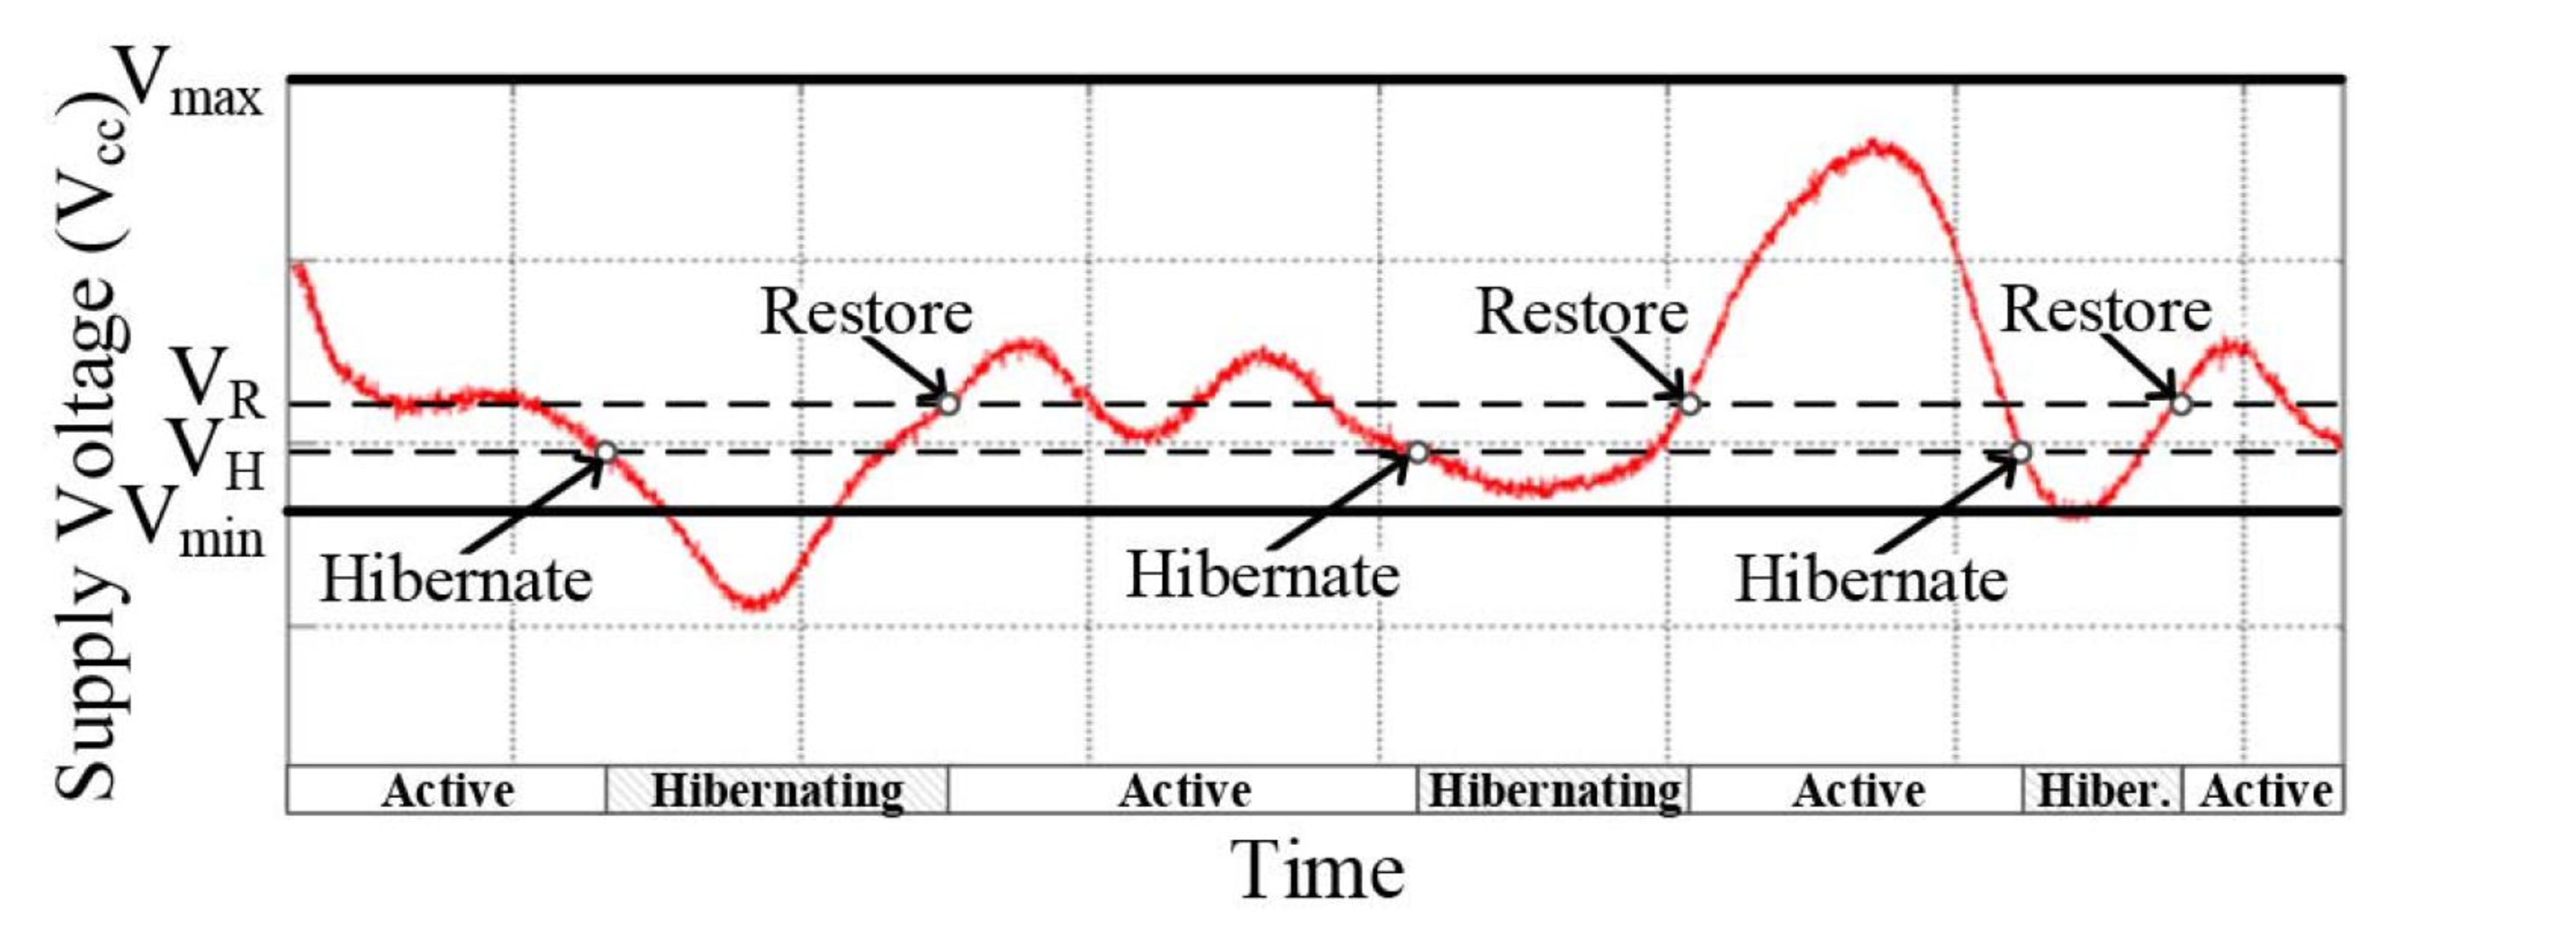
\includegraphics[width=\columnwidth]{ch2_review/figures/hibernus}
    \caption{Voltage trace with hibernation and restoration points in Hibernus (taken from \cite{balsamo2015hibernus}).}
    \label{Figure:hibernus}
\end{figure}

Quickrecall~\cite{jayakumar2014quickrecall} is a similar approach to Hibernus except replacing RAM with NVM, so that all the run-time volatile data become non-volatile and only registers are necessary to be saved in a snapshot. An external voltage comparator detects a triggering voltage $V_{trig}$ to back up only peripherals and registers. Compared to the voltage thresholds in Mementos and Hibernus, $V_{trig}$ in Quickrecall is lower since the reduced energy and time overheads for saving and restoring a snapshot. However, using NVM as RAM may lead to the higher cost of NVM accesses. A comparison between Hibernus and Quickrecall is presented in~\cite{rodriguez2015approaches}, showing that Quickrecall performs worse when the frequency of power interrupts is low as the NVM consumes more than volatile RAM, and performs better when the frequency of power interrupts is high as the overheads of saving snapshots are much lower.

Reactive IC methods only save snapshots when power failure is imminent, and hence, reduce the number of snapshots compared to checkpointing methods. Also, reactive IC avoids code re-execution by suspending execution after saving a snapshot, and hence, ensures idempotency. 

% the size effect of energy buffers on reactive IC
The RAM usage varies at run time, so the size of snapshots in reactive IC also varies throughout code execution. To circumvent this issue, Hibernus saves the entire RAM in each snapshot while Quickrecall does not use RAM at all. Comparing Hibernus to checkpointing methods, the overheads of saving snapshots in Hibernus is larger as checkpointing methods can avoid saving large snapshots by analysing the program. Such high saving overheads becomes significant when the frequency of power outages increases. Increasing the size of energy storage in reactive IC should be helpful to mitigate frequent snapshot taking because the increased energy storage can filter the variations of supply voltage and avoid frequent voltage drops. 

\subsection{Harvest-Store-Use IC}

Harvest-store-use IC systems perform a complete task in one consecutive period when the harvested energy in energy storage is enough. A complete task typically includes sensing, processing, and transmitting actions. In order to sustain a successful task execution, the required capacity of energy storage is larger than the minimum required storage in other IC methodologies. Harvest-store-use systems need to calibrate the energy consumption of the task at design time and set an energy threshold to trigger execution based on that energy consumption. When the threshold is reached, which means there is enough energy for a task, the system performs one task and sleeps until the next threshold trigger. As shown in~\fref{Figure:saveanduse}, the behaviours of the amount of stored energy can be seen as alternating in turn between two states: the collecting state and the executing state.
% These systems work during the sporadic energy bursts.

\begin{figure}
    \centering
    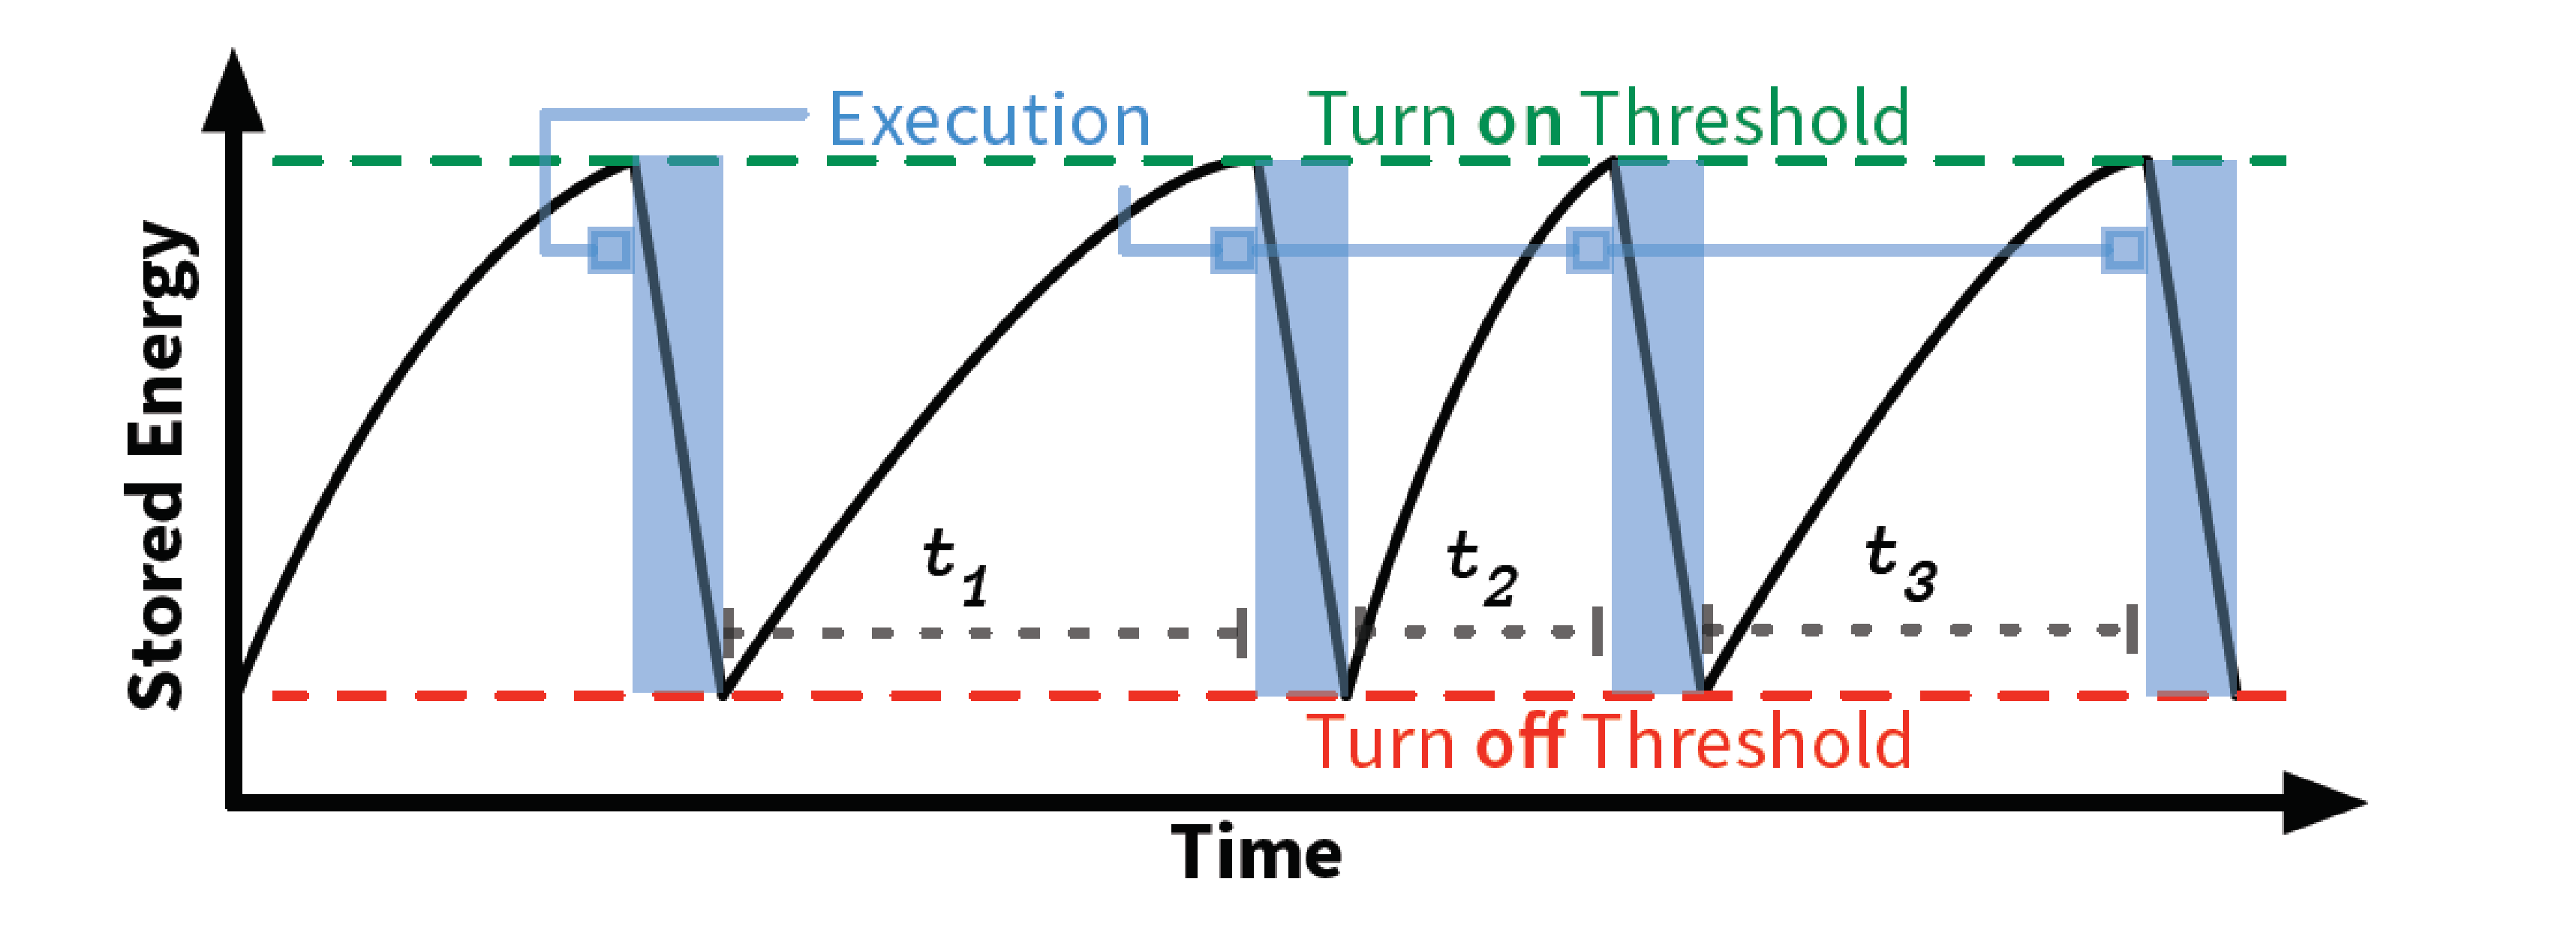
\includegraphics[width=\columnwidth]{ch2_review/figures/saveanduse}
    \caption{Harvest-Store-Use execution (taken from~\cite{hester2017new}).}
    \label{Figure:saveanduse}
\end{figure}

Monjolo~\cite{debruin2013monjolo} is an early design following the harvest-store-use pattern. Monjolo presents a home power meter, whereby a current transformer is installed around the main power cable and provides the energy for this metering system. When the energy stored in a 500$\mu$F capacitor reaches a predefined amount, the system transmits a data packet. Another wireless receiver keeps collecting these packets and approximates the power of the main cable based on the receiving frequency of packets. Such a system contains little sensing and processing work on the transmitting node, and instead, it treats the intensity of energy sources as the sensing data, and processes this translation of data on the receiving node which is powered stably.

WISPCam~\cite{naderiparizi2015wispcam} is a wireless camera that obtains energy from an RF harvester. The harvested energy is stored in a 6mF supercapacitor and the data (photos) are saved in NVM. Once the energy is sufficient for taking one photo, the system starts execution and depletes the energy for taking a picture and data transmission. 

Similarly, Dynamic Energy Burst Scaling (DEBS)~\cite{gomez2016dynamic} also wakes up and executes tasks when there is enough energy in the 80$\mu$F capacitor. The major difference between DEBS and the above two approaches is DEBS can adjust the energy thresholds dynamically for a set of different tasks and generates energy bursts according to which task is in need.

Harvest-store-use paradigms are suitable for occasions where the harvested power is too weak to support the power consumption of any normal execution (other IC methodologies may quickly deplete energy storage and make little progress). Also, harvest-store-use methods circumvent the idempotency issues by complete tasks in one burst. However, this pattern is task-based, which means its operation is limited to one or several fixed energy-defined tasks and also relies on high-quality design-time profiling of tasks.

\subsection{Task-based IC}

% a figure to illustrate task-based IC?
Task-based IC decomposes a program into a series of atomic tasks, which only deliver non-volatile results after all operations in a task are completed~\cite{lucia2015simpler}. Task-based IC is achieved by programming and execution models, which aim to ensure NVM consistency and idempotency. In such models, accesses to NVM and I/O operations are carefully managed to prevent idempotent violations. To ensure idempotency, the program control flow is divided by task boundaries, and the communication between tasks is enabled by reading or writing NVM data on those boundaries. To avoid non-termination, the maximum size of one task is limited by the capacity of energy storage. Therefore, task-based IC can be seen as a rigorously-organized and fine-grained checkpointing method, which eliminates the the non-termination and idempotency problems in checkpointing IC. Task-based systems feature with fast suspend and restore operations because only the runtime and the current task should be versioned and restored through power outages~\cite{sliper2018enabling}. 

DINO~\cite{lucia2015simpler} proposes the first task-based IC programming and execution model, illustrating the task-based idea and providing a basic groundwork. DINO implements the programming and execution model on the LLVM compiler for C code, with program libraries and compiler passes. Chain~\cite{colin2016chain} improves DINO data flows with "Channels", which is dedicated to manage non-volatile data, guaranteeing the correctness on applications with both idempotent and non-idempotent code. Alpaca~\cite{maeng2017alpaca} introduces data privatization which reduces memory usage compared to Chain.

A main drawback of DINO, Chain, and Alpaca is they require great programming efforts for programmers to understand the implemented libraries and redesign a program according to the task-based concept. A recent work, CleanCut~\cite{colin2018termination}, proposes an auxiliary tool to check and automatically decompose the non-terminating tasks (the energy consumption of which exceeds the capacity of system energy storage). 

Also, like checkpointing IC, task-based IC inevitably involves re-execution. Alpaca, the state-of-the-art task-based approach, reports a run time overhead of 1.3-3.6x compared to plain C code given constant power supply. 

\subsection{Non-Volatile Processors}

Non-Volatile Processors (NVPs) incorporate automatic backup and restore hardware within the chips. A comparison of memory architecture between traditional processors and NVPs is shown in~\fref{Figure:nvp}. The traditional volatile elements are replaced with non-volatile elements to achieve efficient backup and restore operations with a faster speed and lower energy consumption than the conventional memory architecture. To be specific, the registers and cache are equipped with built-in additional non-volatile backup and restore circuits, so that when the supply power is going to disappear, the computing state can be saved locally just beside the elements, rather than being copied out into an external NVM. It is reported that the backup and restore speed of NVPs can be 2-4$\times$ magnitudes faster than the state-of-the-art NVM based commercial processors~\cite{liu2015ambient}. 

\begin{figure}
    \centering
    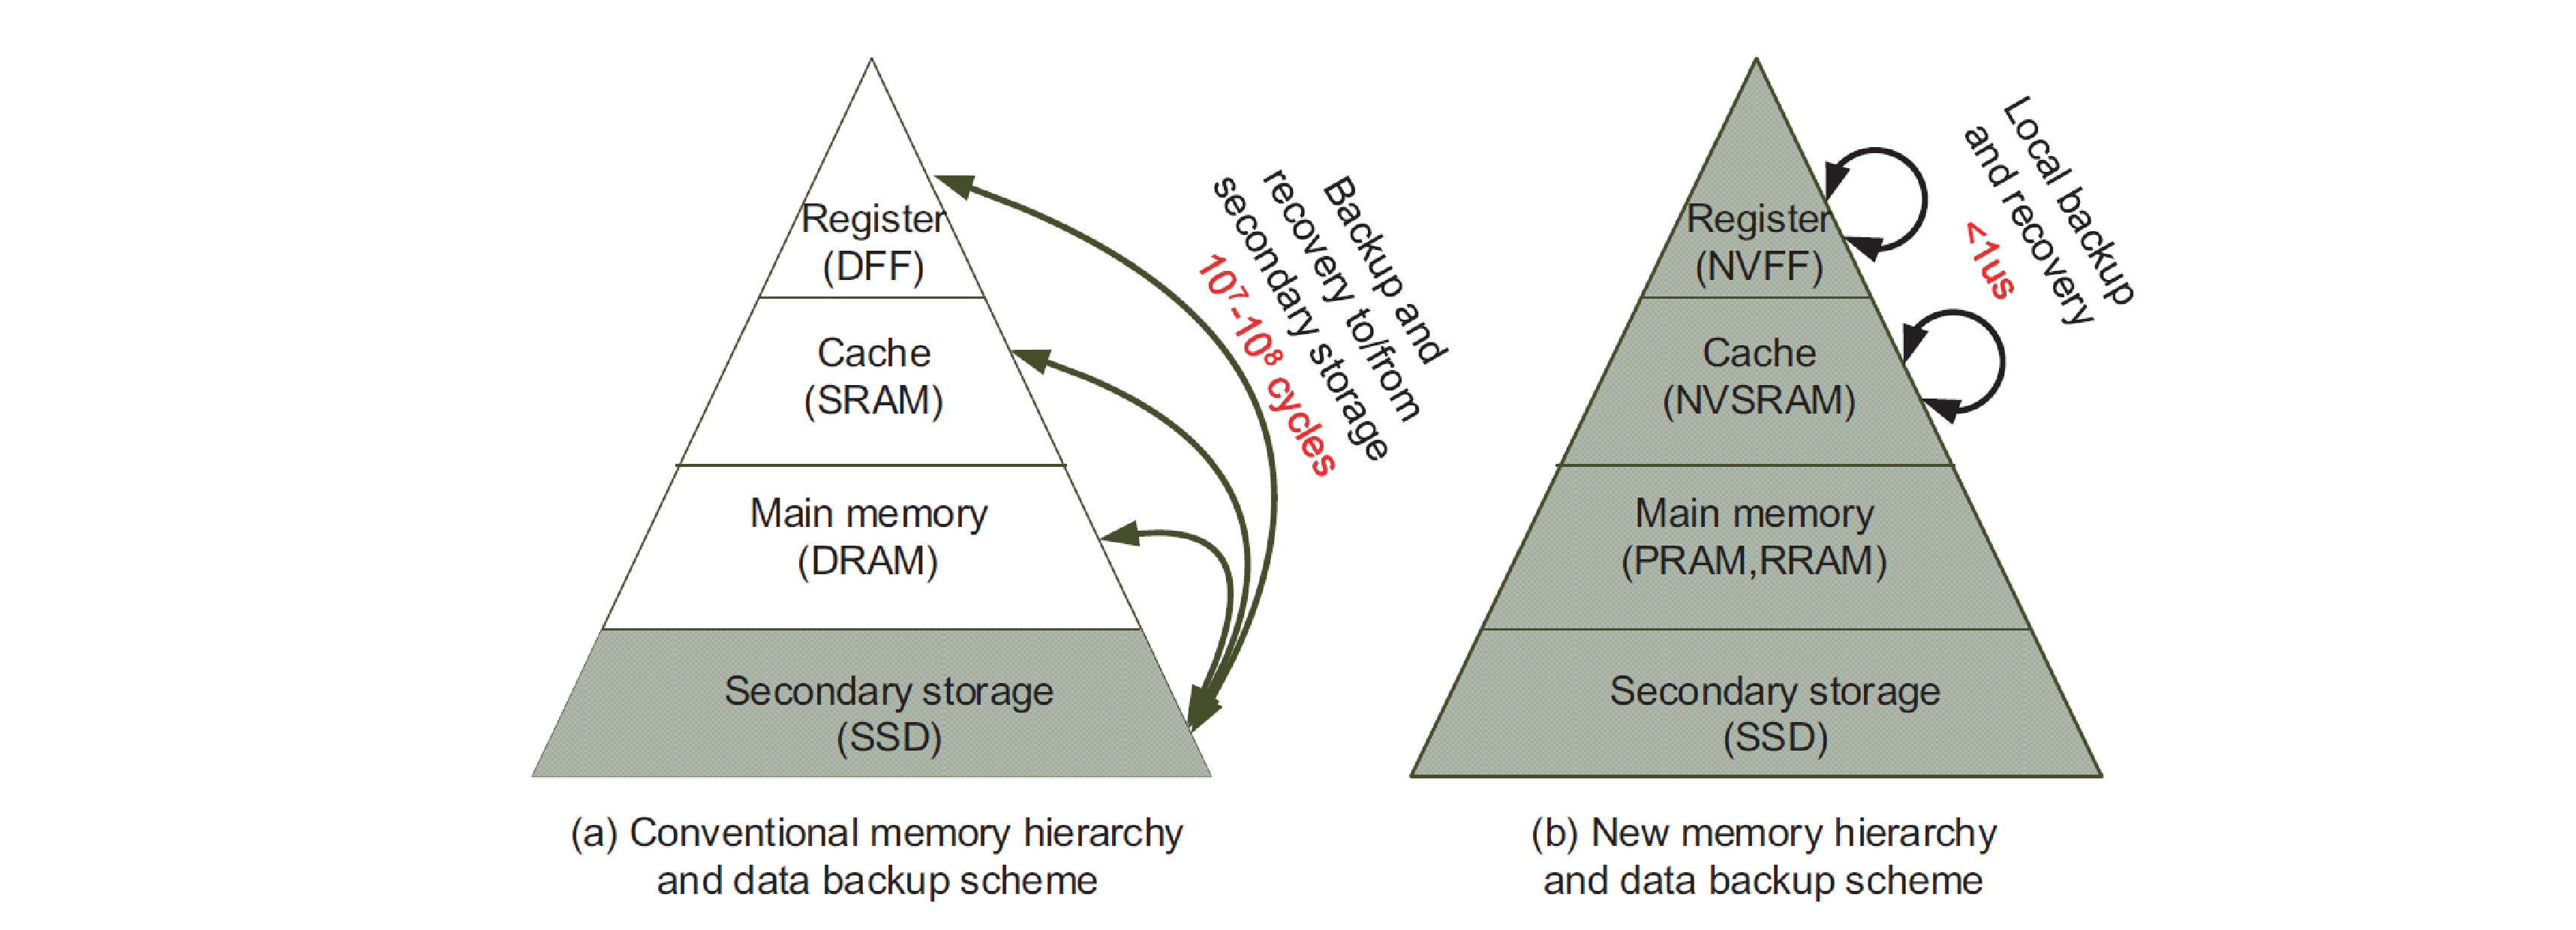
\includegraphics[width=\columnwidth]{ch2_review/figures/nvp}
    \caption{Memory architectures of traditional processors and NVPs (taken from~\cite{liu2015ambient}).}
    \label{Figure:nvp}
\end{figure}

Wang \textit{et al.}~\cite{wang20123us} present a preliminary NVP with 3$\mu$s backup time and 7$\mu$s restore time, which enables the processor to operate safely under a 20 kHz square wave of power. As a comparison, the existing MCUs in TI MSP430 family can only achieve 212$\mu$s and 310$\mu$s for saving and restoring states respectively. Su \textit{et al.}~\cite{su2017ferroelectric} extend the backup and restore time overheads to a system level, presenting a NVP with 46$\mu$s system-level wake-up time and 14$\mu$s system-level sleep time. Liu \textit{et al.}~\cite{liu2019130} integrate a NVP into a system-on-chip with independent backup and restore circuits for peripherals. 

NVP-based research follows with the development of NVP hardware. Ma \textit{et al.}~\cite{ma2015architecture} examine the performance and energy consumption of several types of NVPs with different ambient sources, providing a guideline for NVPs selection. The concept of "Incidental Computing" based on NVPs is proposed in~\cite{ma2017incidental} to improve the forward progress under unstable power supply, and also provides an evaluation of performance on NVPs. Essentially, it pays more attention to processing forward data in need than the buffered historical data from recovery, but an incidental recomputing on the historical data is performed when there is abundant energy. It is reported that this approach outperforms the existing save-and-use computing scheme by 2.2-5$\times$ in the simulation with respect to an image processing speed, and also the forward progress is improved by 4.28$\times$ on average over a basic NVP.

NVPs perform well in terms of the response to power intermittency, but the research on how to deliver better forward progress with NVPs is limited. Dynamic Voltage and Frequency Scaling (DVFS) can be a potentially applicable solution~\cite{ma2016nonvolatile}. In a traditional NVP, the small buffering capacitor tends to be either charged to be full or depleted rapidly and frequently~\cite{su2017nonvolatile}. This behaviour accounts for a large part of backup and recovery overheads, so power management based on NVP is in need.

\section{Power-Neutral Computing} \label{Section:PN}

While IC aims to ensure forward execution despite frequent power outages, energy harvesters may also generate more power than systems can consume when ambient sources are sufficient. Such excessive energy is wasted if not stored for later usage or consumed immediately. 
% Adaptive computing in energy harvesting computing denotes energy management techniques that aim to efficiently utilise the harvested energy. 
% Different sizes of storage supports different scale of energy management.

\subsection{Principles of Operations}

Power-neutral (PN) computing aims to manage power without additional storage or with only a very limited amount of storage which can only sustain its system for milliseconds. In principle, power-neutral computing is a special case of energy neutral computing when $\Delta t$ in Equation~\ref{eq:energyneutral} is equal (or close) to zero. Technically, PN computing scales the instantaneous system power consumption to match the instantaneous harvested power with theoretically zero storage (in other words, energy neutrality is met instantaneously). PN operations can be translated into the following expressions:

\begin{equation} \label{eq:pn}
    P_h(t) = P_c(t)
\end{equation}
\begin{equation} \label{eq:pnon}
    where\quad t \in \{t|V_{cc}(t) \geq V_{min}\}
\end{equation}

where $V_{cc}$ is the input voltage of the computing load, and $V_{min}$ is the minimum voltage required for the system to operate. Equation~\ref{eq:pn} describes the methodology of power neutrality (dynamic and instantaneous power adaptation). Equation~\ref{eq:pnon} limits the requirement for power neutrality that the system should be powered and active to make reactions of performance scaling. This requirement may change according to different system designs, but for contemporary computing and sensing loads, this is determined by the supply voltage. 

Given a very limited amount of storage and a range of scalable performance and power consumption, PN computing scales down performance if $P_h$ is lower than $P_c$, such that $V_{cc}$ remains stable, which extends execution time and avoids suspend and restore operations. On the other hand, PN computing scales up performance if $P_h$ is higher than $P_c$, such that the excessive harvested energy is immediately consumed on useful work rather than wasted.

In practice, however, there does not exist a system that can adjust its power consumption instantaneously to the harvested power without any overheads. Any performance scaling costs a small amount of time and energy overheads, which a system cannot afford without any energy storage. Therefore, a minimum storage is still required, normally in the form of decoupling or parasitic capacitance, to provide a small but sufficient amount of energy for scaling performance and adapting power consumption.
% In practice, a PN system tries to meet Equation~\ref{eq:pn} as quickly as possible while switching overheads still exist.
% switching granularity/resolution?

In order to achieve power neutrality, a system has to adapt its performance and hence power consumption. Performance scaling can be achieved by hardware controlling, such as Dynamic Frequency Scaling (DFS)~\cite{balsamo2016graceful}, Dynamic Voltage and Frequency Scaling (DVFS)~\cite{fletcher2017power}, or switching on/off load elements~\cite{wang2016storage, fletcher2017power} (also known as Dynamic Power Management, DPM~\cite{lu2000low} or hot-plugging). Apart from these achieved methods, duty-cycle scaling and task scheduling are also choices for changing performance and consumption, though they have not been implemented in current research yet.

\subsection{Recent Approaches}

The concept of PN computing is proposed in~\cite{balsamo2016graceful} and implemented on a Texas Instrument MSP430FR5739 MCU without an external energy buffer. As shown in~\fref{Figure:graceful_schematic}, the executing load is directly connected to a regulated energy harvesting source. The control scheme in~\cite{balsamo2016graceful} utilises DFS with a voltage feedback. Specifically, two voltage thresholds, $V_{dec}$ and $V_{inc}$, are set for detecting voltage variance caused by power inequality and then scaling performance accordingly. In order to respond fast to power difference, the capacitance is reduced to 19$\mu$F, which is only the parasitic and on-board decoupling capacitance. When $P_h(t) > P_c(t)$ and the operating voltage $V_{cc}$ increases rapidly due to the small capacitance and reaches $V_{inc}$, the MCU increases its operating frequency resulting in faster computing speed and higher power consumption, and also increases the thresholds between which the new voltage value is contained; and vice versa, a reverse procedure is executed for $P_h(t) < P_c(t)$. In a word, this control scheme is trying to make the operating voltage stable around a desired value so that $P_h(t)$  equals $P_c(t)$ approximately.

\begin{figure}
    \centering
    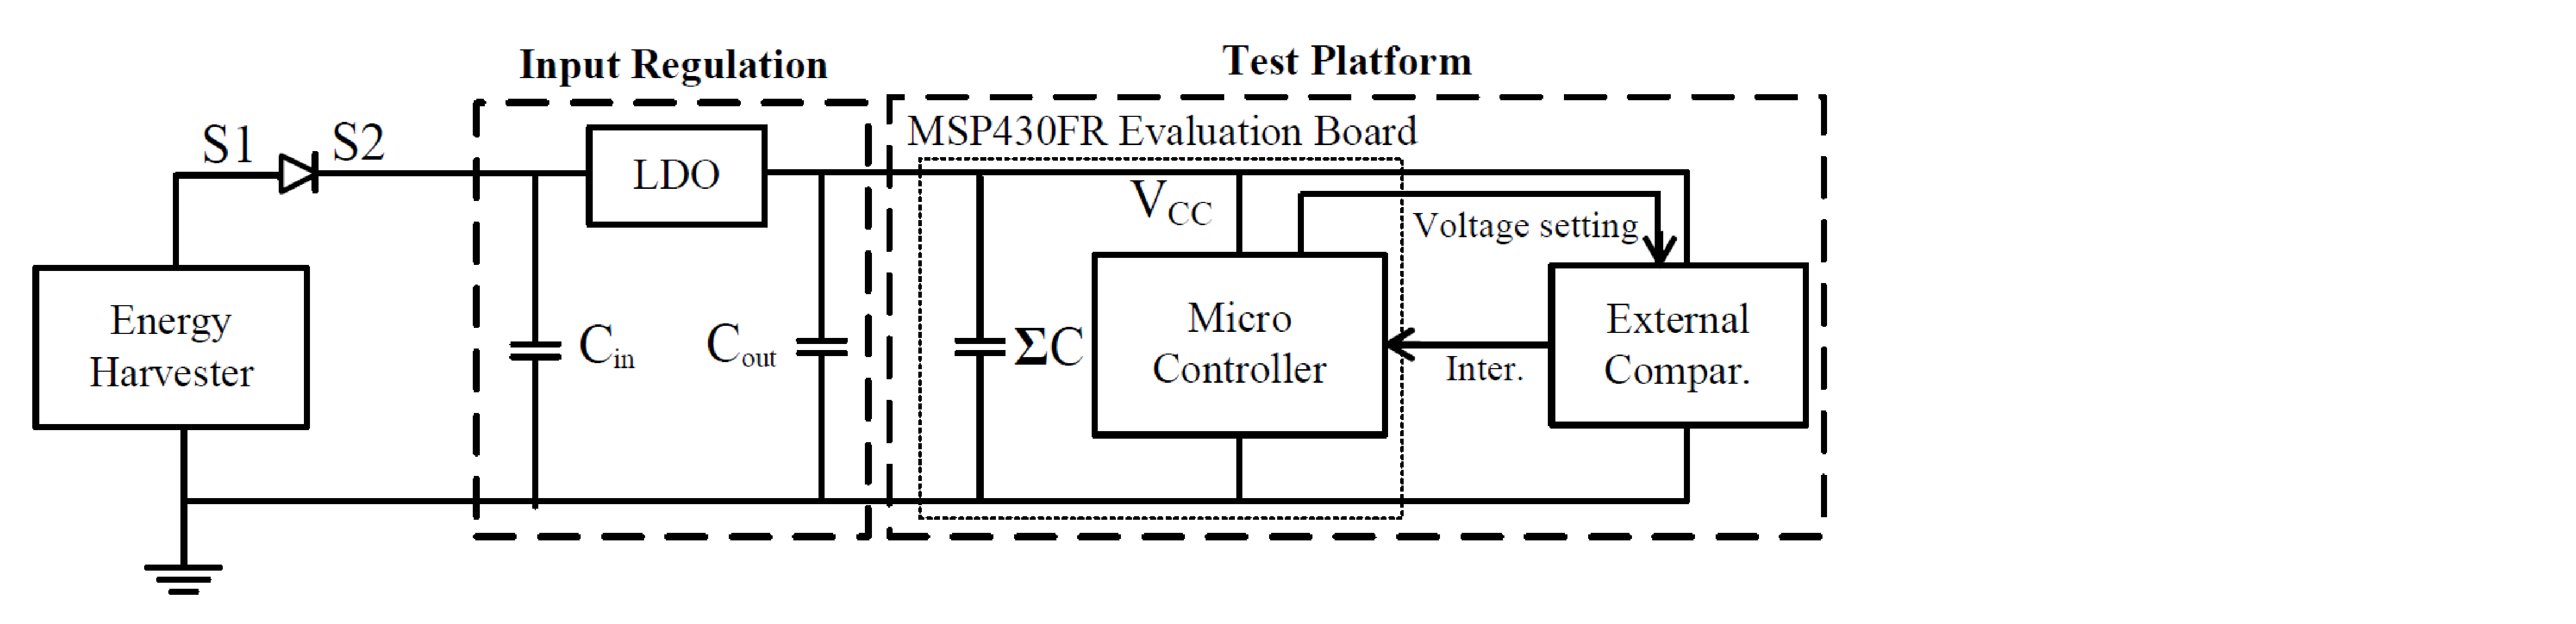
\includegraphics[width=\columnwidth]{ch2_review/figures/graceful_schematic}
    \caption{Architecture of an example power neutral system based on TI MSP430FR platform (taken from \cite{balsamo2016graceful}).}
    \label{Figure:graceful_schematic}
\end{figure}
%flowchart of this control scheme is present in figure?

A similar control scheme is adopted in~\cite{fletcher2017power} where the platform is an MP-SoC adopting DVFS and DPM, which leads to higher performance, higher power consumption, and more operating points than the MCU in~\cite{balsamo2016graceful}. A 47mF supercapacitor is used for safely overcoming performance switching where the power consumption of the board is normally above 2W. As an illustration for how to scale performance by DVFS and DPM, \fref{Figure:dvfs} presents an example application profile of 'power consumption vs performance' when DVFS and DPM applied on a heterogeneous multi-processor system-on-chip (MP-SoC) platform. The SoC used in this platform is the Samsung Exynos5422 big.LITTLE SoC with four 'big' high-performance A15 cores and four 'LITTLE' low-power A7 cores. In this case, the performance refers to the speed of executing this application for one time and is proportional to the operating frequency under a certain core configuration. As shown in the figure, each performance level (a pair of frequency and core status, also named as an operating point) requires a certain power consumption. At run-time, the system dynamically switch its performance among these operating points so as to timely match $P_c(t)$ with $P_h(t)$.

\begin{figure}
    \centering
    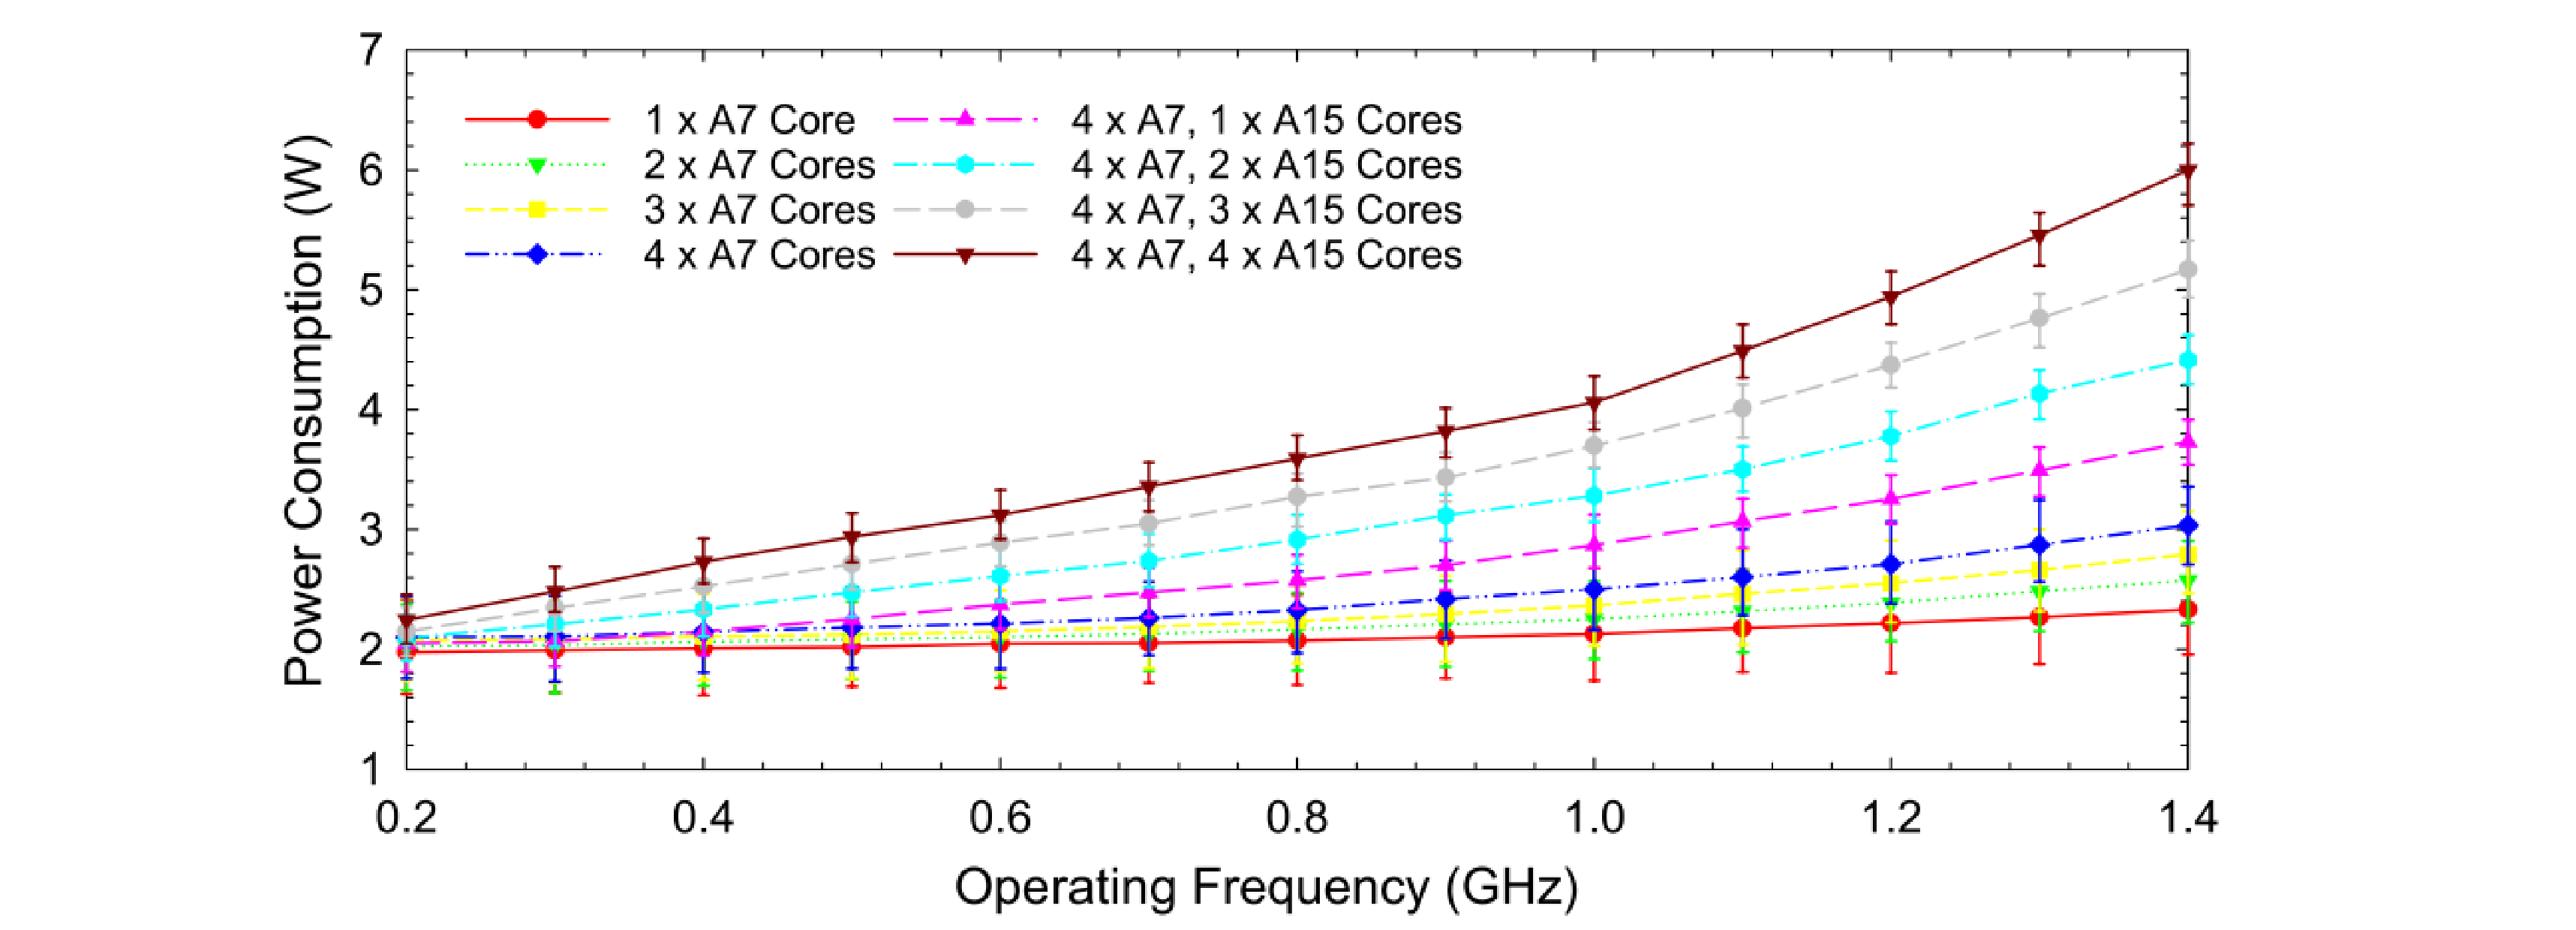
\includegraphics[width=\columnwidth]{ch2_review/figures/dvfs}
    \caption{Board power consumption of ODROID XU4 vs operating frequency and core configurations, running CPU intensive application Raytrace (taken from \cite{fletcher2017power}).}
    \label{Figure:dvfs}
\end{figure}

There are three advantages in this kind of PN control scheme. First, the voltage is stabilized so it can offset ephemeral power drops which cause insufficient voltage supply and power failures, and therefore the lifetime increases (e.g. reported by 4-88\% in~\cite{balsamo2016graceful}). Second, as power neutral computing eliminates many elements that required in EN systems, such as large energy storage, power converters and MPPT units, the size and cost of devices is reduced and the number of power consumption components also decreases. Third, if powered by a solar panel and the operating voltage range encompasses the MPP of the given solar panel, the system embraces an intrinsic MPPT characteristic as it can stabilize the voltage around a target value.

Similarly, Wang \textit{et al.}~\cite{wang2016storage} propose a storage-less and converter-less approach which can be classified as a power neutral system. In this design, a 47$\mu$F bulk capacitor is equipped with a 3.29mW non-volatile MCU and up to 16.5mW peripherals. This capacitor is also small enough compared to the 19$\mu$F capacitance operating with an up to 3 mW MCU in~\cite{balsamo2016graceful}. An external MPPT controlling element dynamically adjusts the power duty-cycle for the non-volatile load in order to match the harvested current and the consumed current, and hence power neutrality is met. 

One disadvantage of power neutral computing is that it has to passively scale its power consumption as well as its performance, causing large variations in performance. However, this might not be good in terms of the overall forward progress. In the next chapter, a preliminary analyse is explained about how the forward progress is improved when the capacitor size is increased, while not violating the merits of PN computing. 